\documentclass[14pt]{extarticle}
\usepackage{ragged2e}  % для выравнивания текста
\usepackage{float}  % для управления расположением фигур
\usepackage[bottom=1cm,right=1cm,left=2cm]{geometry}
\usepackage{graphicx}

% Russian-specific packages
%--------------------------------------
\usepackage[T2A,T1]{fontenc}
\usepackage[utf8]{inputenc}
\usepackage[english,russian]{babel}
%--------------------------------------
\usepackage{amsfonts}       % blackboard math symbols
\usepackage{xurl}
%\usepackage[backend=biber]{biblatex}
\usepackage[backend=biber, style=gost-numeric, language=auto, autolang=other]{biblatex}
\usepackage{breakurl}

\addbibresource{references.bib}

% Настройка для переноса URL-адресов
\setcounter{biburllcpenalty}{9000} % URL не могут быть разорваны на строчные буквы
\setcounter{biburlucpenalty}{9000} % URL не могут быть разорваны на заглавные буквы
\setcounter{biburlnumpenalty}{9000} % URL не могут быть разорваны на цифры

% Настройка стиля библиографии для уменьшения размера шрифта
\renewcommand*{\bibfont}{\scriptsize}

\setlength{\topmargin}{-2cm}

\renewcommand{\baselinestretch}{2}
\newcommand{\namesigdate}[2][5cm]{%
    \begin{minipage}{#1}
    #2 \vspace{1.5cm}\hrule\smallskip
    \end{minipage}}

\begin{document}


\pagenumbering{gobble}

\begin{titlepage} % Suppresses displaying the page number on the title page and the subsequent page counts as page 1
\fontsize{12pt}{10pt}\selectfont
\newcommand{\HRule}{\rule{\linewidth}{0.5mm}} % Defines a new command for horizontal lines, change thickness here

\center % Centre everything on the page

%------------------------------------------------
%   Headings
%------------------------------------------------


\textsc{ФЕДЕРАЛЬНОЕ ГОСУДАРСТВЕННОЕ АВТОНОМНОЕ}\\
\textsc{ОБРАЗОВАТЕЛЬНОЕ УЧРЕЖДЕНИЕ ВЫСШЕГО ОБРАЗОВАНИЯ}\\
\textsc{«НАЦИОНАЛЬНЫЙ ИССЛЕДОВАТЕЛЬСКИЙ УНИВЕРСИТЕТ}\\
\textsc{«ВЫСШАЯ ШКОЛА ЭКОНОМИКИ»}\\
\textsc{\bfseries Московский институт электроники и математики}\\[1.5cm]

\textsc{Морозов Денис Сергеевич}\\
\textsc{\large\bfseries Моя первая нейронная сеть. Определение марки автомобиля по фотографии} % Major heading such as course name

\vfill\vfill
\textsc{Проектная работа}\\
\textsc{студента образовательной программы бакалавриата}\\
\textsc{«Прикладная математика»}\\
\textsc{по направлению подготовки 01.03.04 ПРИКЛАДНАЯ МАТЕМАТИКА}\\[1.5cm]

%------------------------------------------------
%   Date
%------------------------------------------------

\begin{flushright}
Студент\\
Д. С. Морозов
\end{flushright}
\hfill
\begin{minipage}{0.45\textwidth}
    \begin{tabular}{p{\textwidth}}
    \begin{flushright}
    Руководитель проектной работы\\
    Доктор физико-математических наук, профессор\\
    Попов Виктор Юрьевич\\[0.5cm]
    \end{flushright}
    \end{tabular}
\end{minipage}%

\vfill\vfill\vfill\vfill % Position the date 3/4 down the remaining page

{\large\bfseriesМосква \the\year г.} % Date, change the \today to a set date if you want to be precise

\end{titlepage}

\pagenumbering{arabic}

\tableofcontents % Автоматически формируемое оглавление

\section{Аннотация}

В рамках данного проекта разрабатывалась модель нейронной сети для решения задачи с определением марки автомобиля с использованием языка программирования Python. Были протестированны несколько  модель, способные прогнозировать правильные классы автомобилей. Средняя абсолютная ошибка на тестовых данных составила 1/30 фото. Это неплохой показатель, учитывая небольшой размер датасета и большое количество существующих машин. 

\section{Введение}
\setlength{\parindent}{1cm}  % Установка отступа в начале абзацев
\hspace{1cm}Искусственный интеллект и машинное обучение, в частности глубокие нейронные сети, стали важными инструментами в распознавании изображений. Современные методы машинного обучения позволяют решать сложные задачи анализа и прогнозирования, обеспечивая высокую точность и надежность результатов. Этот проект рассматривает разработку и применение модели нейронной сети для решения задачи классификации изображений, что представляет собой одну из наиболее востребованных задач в области искусственного интеллекта и машинного обучения. В данном отчете подробно рассматриваются этапы создания, обучения и тестирования модели, а также полученные результаты и возможности их улучшения.

Проект выполнялся на языке программирования Python, используя среду разработки Pycharm и современные инструменты и библиотеки, такие как PyTorch Lightning\footnote{\citeauthor{youtubevideo}. \emph{\citetitle{youtubevideo}}.} для упрощения процесса обучения модели и архитектура EfficientNet\footnote{\citeauthor{paperswithcode}. \emph{\citetitle{paperswithcode}}.}, которая отличается высокой производительностью и экономичностью.

EfficientNet использует стратегию компаундного масштабирования для сбалансированного увеличения глубины, ширины и разрешения сети, что позволяет добиться лучших результатов с меньшими вычислительными затратами.
Так же использовался ChatGPT для предотвращения ошибок и кофликтов библиотек\footnote{\citeauthor{chatgpt}. \emph{\citetitle{chatgpt}}.}

\section{Обзор литературы и технологий}
\setlength{\parindent}{1cm} 
\subsection{Обзор нейронных сетей для распознавания изображений}
\hspace{1cm}Глубокие нейронные сети, особенно сверточные (CNN), показали высокую эффективность в задачах распознавания изображений. CNN состоят из слоев свертки и объединения, которые позволяют автоматически выделять признаки из изображений. 

Основные компоненты нейронной сети включают входной слой, несколько скрытых слоев и выходной слой. Каждый нейрон в скрытом слое выполняет нелинейное преобразование данных, что позволяет модели обучаться сложным зависимостям между входными и выходными данными.

\subsection{Сравнение различных архитектур CNN}
\hspace{1cm}Мной были рассмотрены архитектуры, такие как ResNet50\footnote{\citeauthor{resnet50hub}. \emph{\citetitle{resnet50hub}}.}, Resnet152\footnote{\citeauthor{resnet152}. \emph{\citetitle{resnet152}}.} и EfficientNet. В последние годы глубокое обучение и нейронные сети стали основным инструментом для решения задач классификации изображений. Одной из самых эффективных архитектур, предложенных в последние годы, является EfficientNet, которая оптимизирует количество параметров и вычислительных ресурсов, сохраняя высокую точность модели. 

\section{Данные и их подготовка}
\subsection{Источники данных}
\hspace{1cm}Для обучения модели использован датасет, содержащий фотографии автомобилей различных марок, собранные из открытых источников, таких как интернет-ресурсы, а именно Kaggle\footnote{\citeauthor{stanfordcars}. \emph{\citetitle{stanfordcars}}.}
. Для подготовки данных использовались библиотеки torchvision и albumentations. Датасет содержал изображения автомобилей, которые были разделены на тренировочные и тестовые наборы.
\begin{figure}[H]
    \centering
    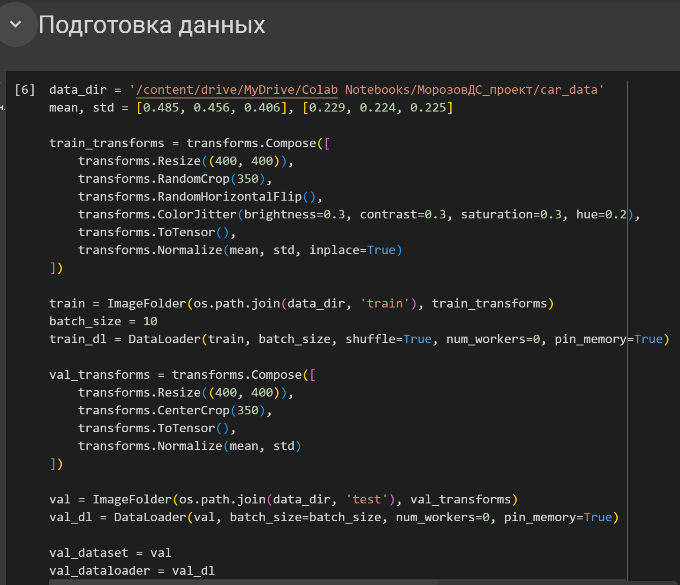
\includegraphics[width=10cm]{images/1.png}
    \caption{Подговка данных}
    \label{fig:10}
\end{figure}

\subsection{Аугментация данных}
\hspace{1cm}Для увеличения объема данных и улучшения обобщающей способности модели использовались техники аугментации, включая вращение, изменение масштаба, случайные обрезки, горизонтальные отражения и изменение яркости, контраста, насыщенности и отражение изображений.

\begin{figure}[H]
\centering
\begin{minipage}{0.49\textwidth}
  \centering
  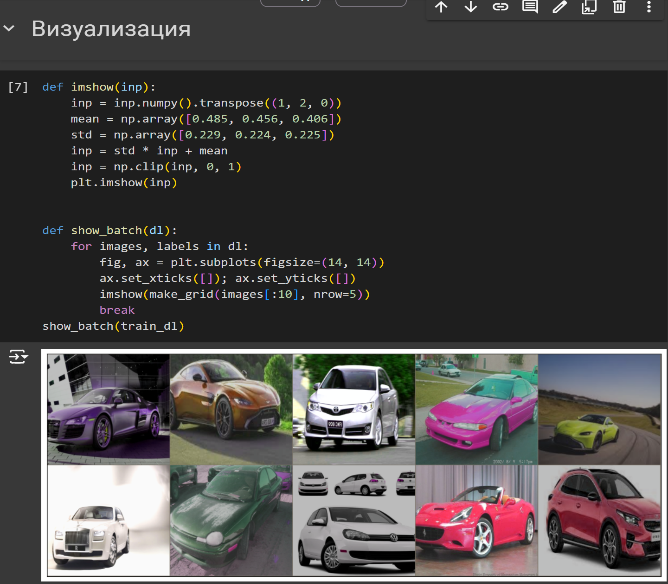
\includegraphics[height=7.1cm]{images/2.png}  
  \caption{Альбументация}
  \label{fig:12}
\end{minipage}
\hfill
\begin{minipage}{0.49\textwidth}
  \centering
  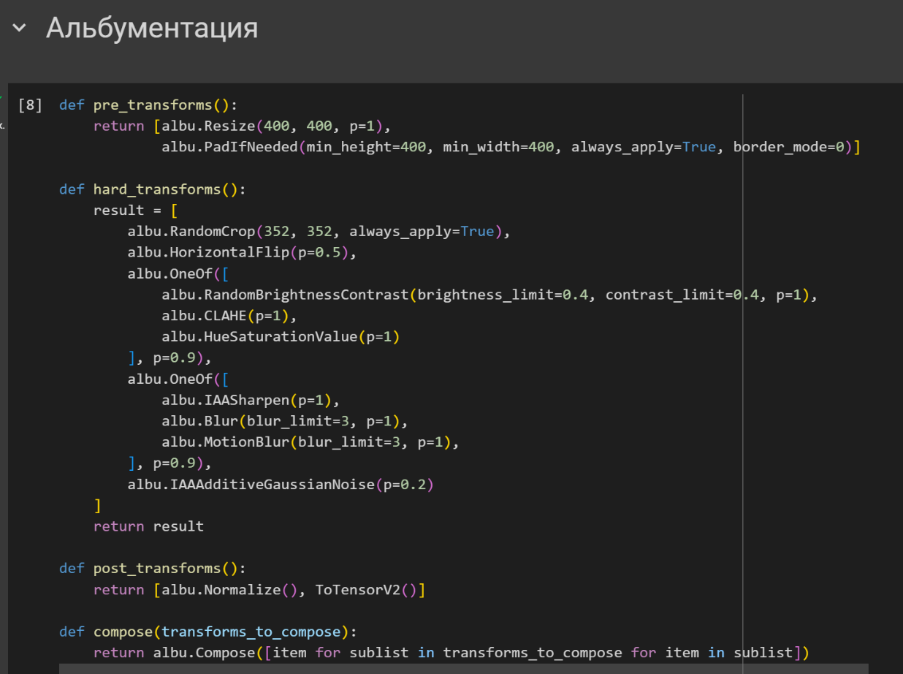
\includegraphics[height=7.1cm]{images/3.png}  
  \caption{Визуализация}
  \label{fig:13}
\end{minipage}
\end{figure}

\subsection{Разделение данных}
\hspace{1cm}Данные были разделены на обучающую и тестовую выборки в соотношении 55/45. Это позволяет оценивать модель на данных, которые она не видела во время обучения.


\begin{figure}[H]
\centering
\begin{minipage}{0.49\textwidth}
  \centering
  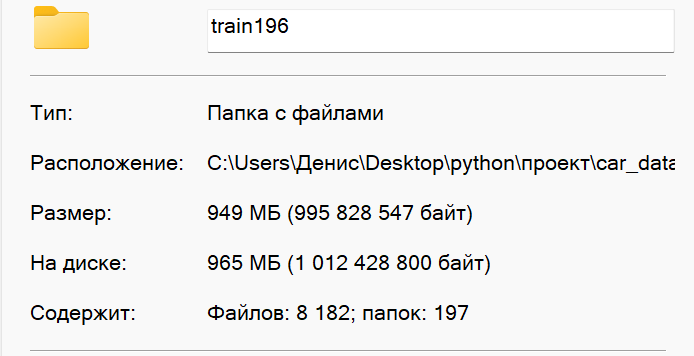
\includegraphics[height=6cm]{images/4.png}  
  \caption{Папка с обучающими данными}
  \label{fig:12}
\end{minipage}
\hfill
\begin{minipage}{0.49\textwidth}
  \centering
  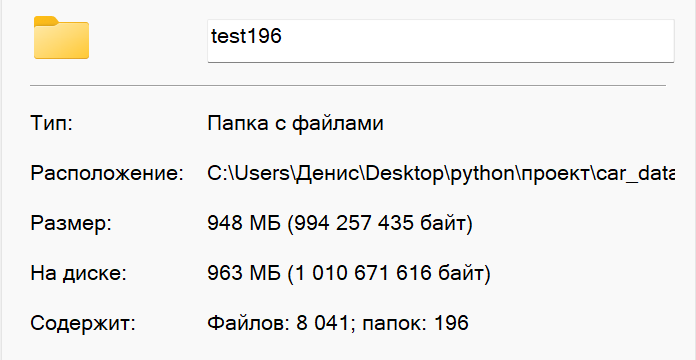
\includegraphics[height=5cm]{images/5.png}  
  \caption{Папка с валидационными данными}
  \label{fig:13}
\end{minipage}
\end{figure}

\section{Архитектура нейросети}
\subsection{Выбор архитектуры}
\hspace{1cm}Наиболее подходящая конфигурация сети определялась экспериментально, с учетом факторов таких как глубина сети, количество фильтров и размер ядра свертки. Так же были настроены логирование с использованием W\&B\footnote{\citeauthor{wandb}. \emph{\citetitle{wandb}}.}, контроль точки модели и ранняя остановка.
\begin{figure}[H]
\centering
\begin{minipage}{0.49\textwidth}
  \centering
  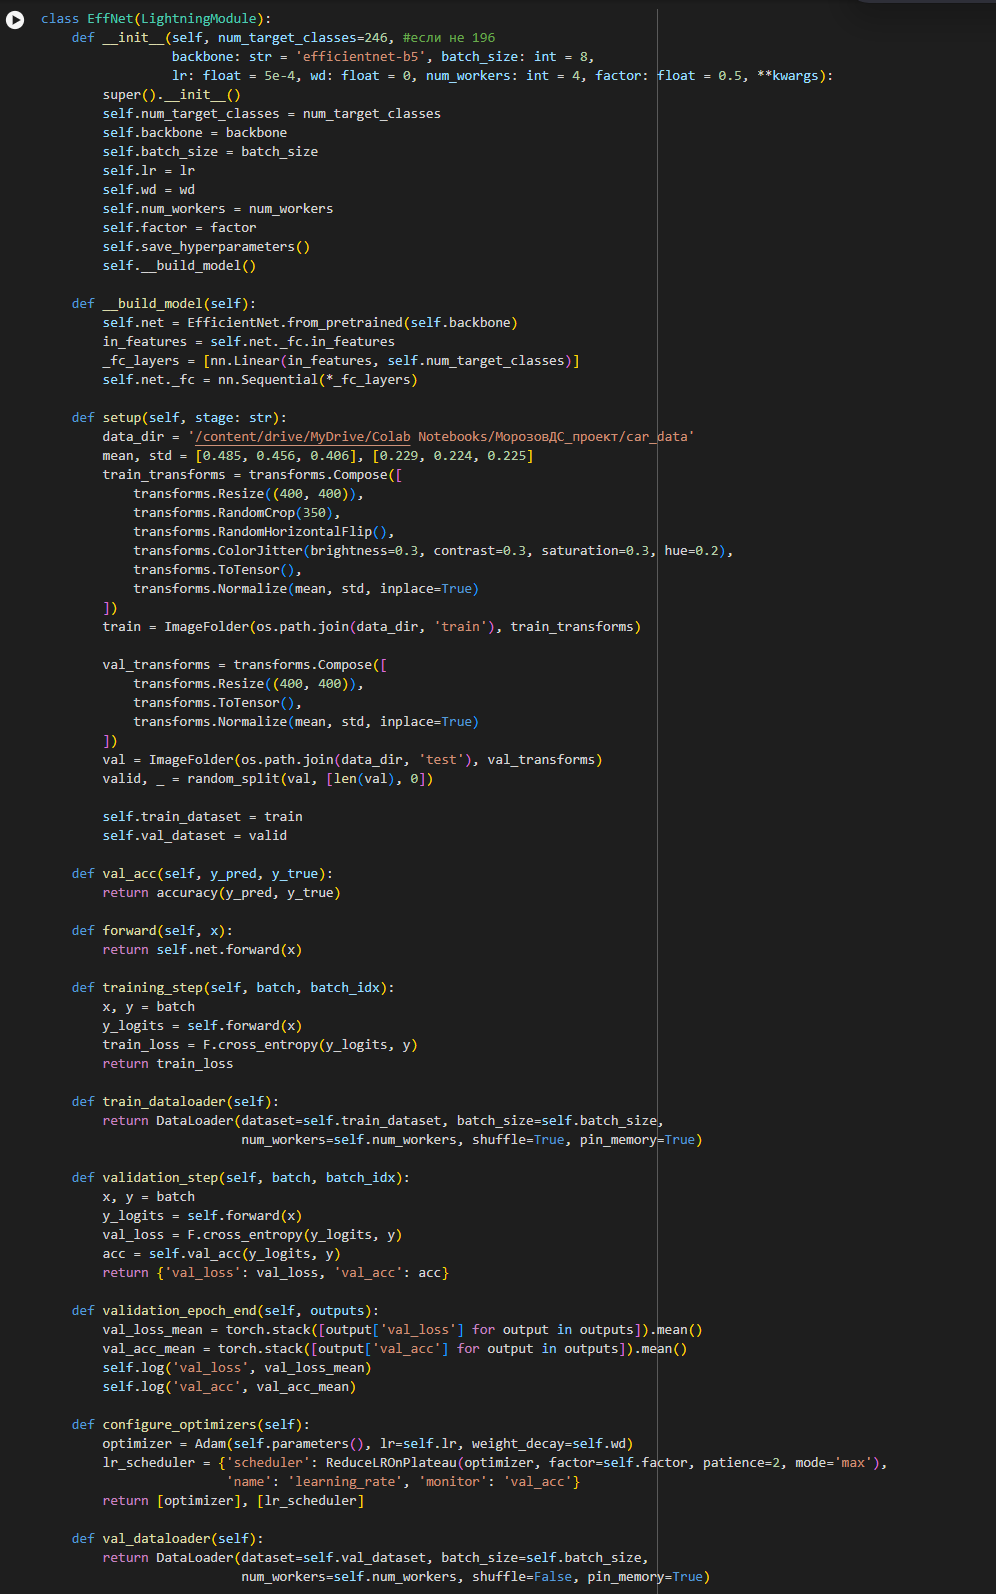
\includegraphics[height=20cm]{images/6.png}  
  \caption{Модель EfficientNet}
  \label{fig:12}
\end{minipage}
\hfill
\begin{minipage}{0.49\textwidth}
  \centering
  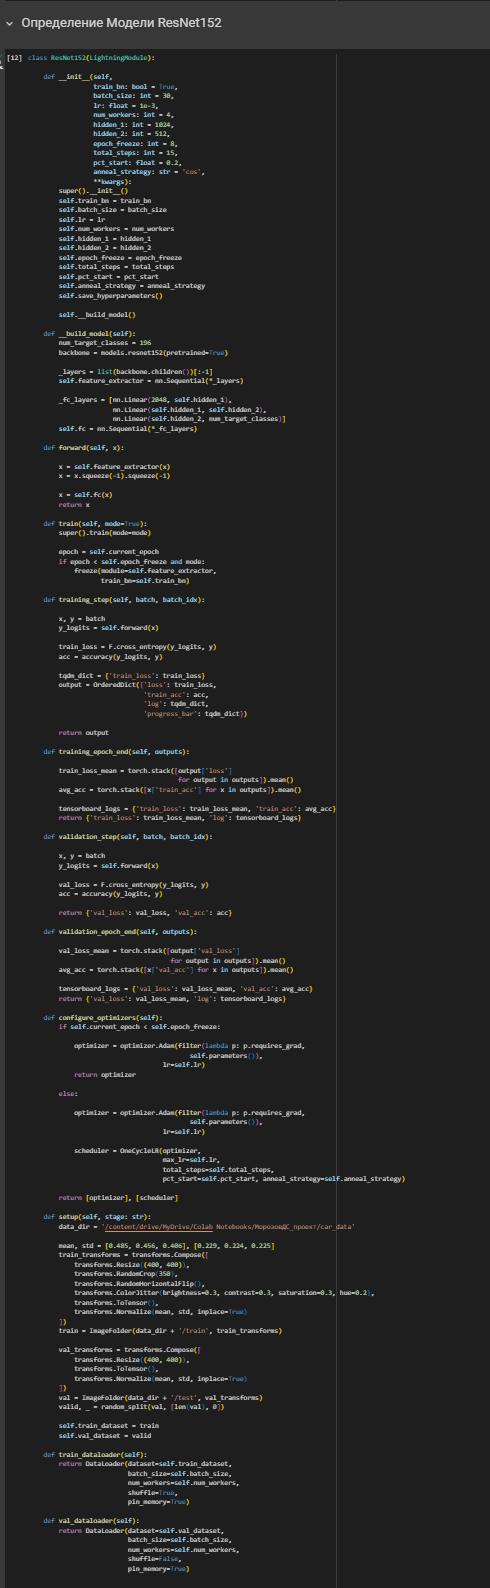
\includegraphics[height=20cm]{images/7.png}  
  \caption{Модель ResNet}
  \label{fig:13}
\end{minipage}
\end{figure}

\subsection{Детали реализации}
\hspace{1cm}Модель состоит из нескольких свёрточных слоев, за которыми следуют слои max-pooling и полносвязные слои. Каждый свёрточный слой использует ReLU (Rectified Linear Unit) в качестве функции активации.
Так же использовал графический процессор\footnote{\citeauthor{youtubegpu}. \emph{\citetitle{youtubegpu}}.} для ускорения обучения с помошью графических ядер\footnote{\citeauthor{pytorchgpu}. \emph{\citetitle{pytorchgpu}}.}.

\section{Обучение модели}
\subsection{Настройка гиперпараметров}
\hspace{1cm}Гиперпараметры, такие как скорость обучения, размер батча и количество эпох, были настроены с использованием методов поиска по сетке и случайного поиска. Начальная скорость обучения установлена на 1e-4, размер батча — 32, количество эпох — 50.
\begin{figure}[H]
    \centering
    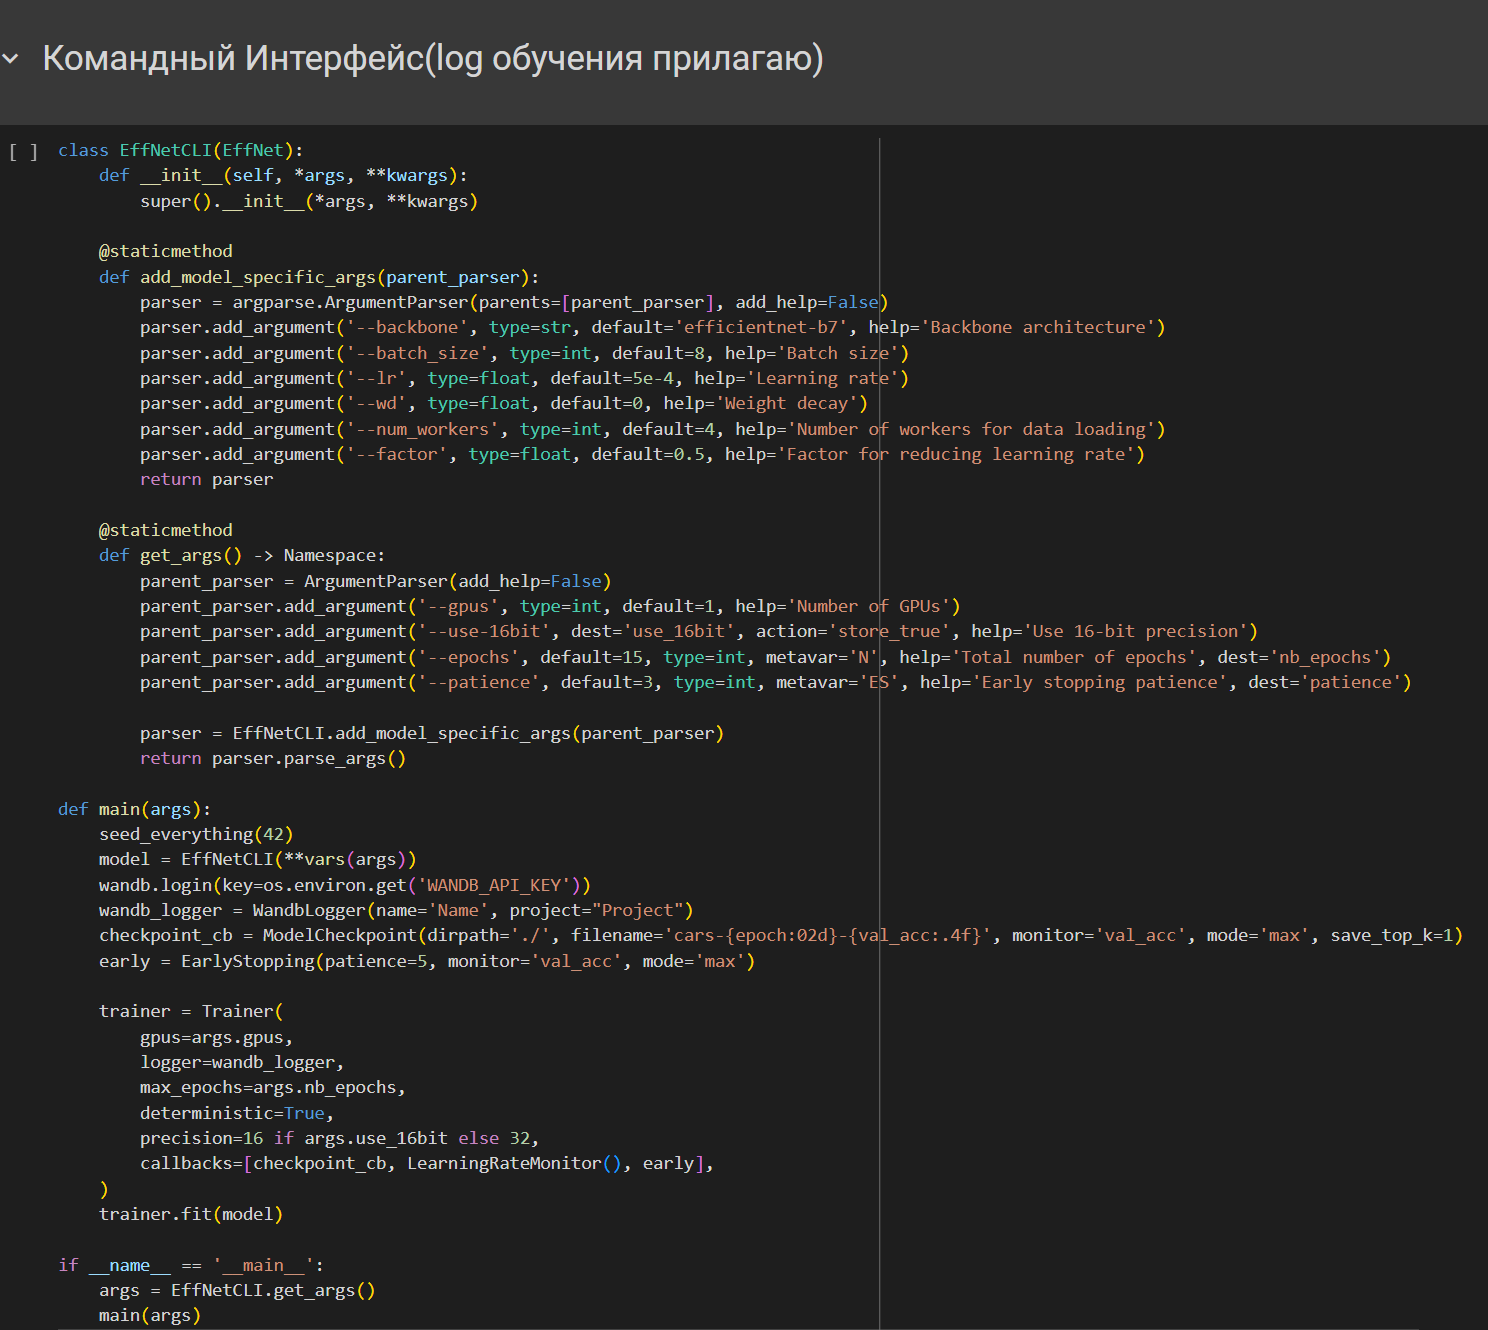
\includegraphics[width=12cm]{images/8.png}
    \caption{Настройка гиперпараметров}
    \label{fig:10}
\end{figure}

\subsection{Использование функции потерь}
\hspace{1cm}Для задачи классификации использовалась кросс-энтропийная функция потерь, которая хорошо подходит для многоклассовых задач.

\subsection{Процесс обучения и валидации}
\hspace{1cm}Процесс обучения включал регулярную валидацию модели на отдельном наборе данных для предотвращения переобучения. Переобучение (overfitting) — это проблема, возникающая, когда модель хорошо работает на тренировочных данных, но показывает плохие результаты на новых, невиданных данных. Для борьбы с переобучением используются следующие методы:
\begin{itemize}
    \item Регуляризация: включает добавление штрафа за сложность модели в функцию потерь. Одним из популярных методов является L2-регуляризация.
    \item Dropout: метод, при котором случайно отключается часть нейронов в процессе обучения, что улучшает обобщающую способность модели.
    \item Кросс-валидация: разделение данных на несколько частей и многократное обучение модели на различных комбинациях этих частей.
\end{itemize}

\section[Результаты и обсуждение]{\textbf{Результаты и обсуждение}}
\subsection[Анализ результатов]{\textbf{Анализ результатов}}

\hspace{1cm}Модель \foreignlanguage{english}{ResNet}50 достигла точности 75\% на тестовом наборе данных. Анализ показал, что модель
хорошо распознаёт популярные марки автомобилей, но испытывает трудности с менее распространёнными марками.

\begin{figure}[H]
\centering
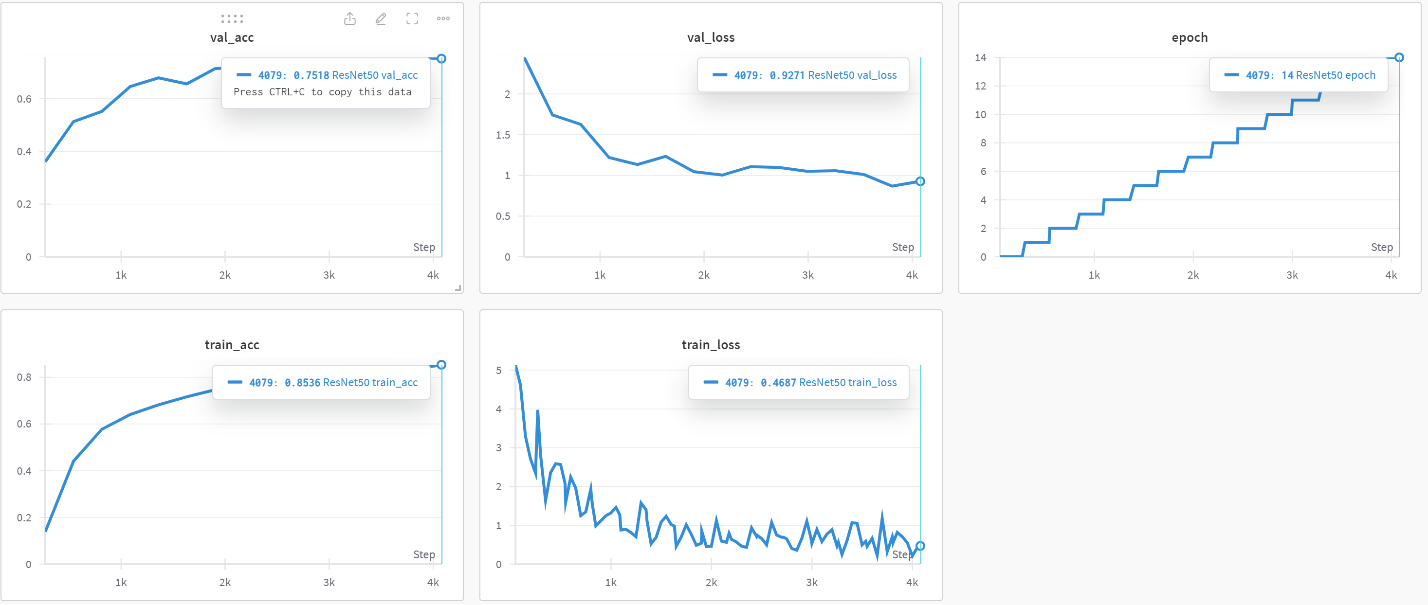
\includegraphics[width=\textwidth]{images/9.png}
\caption{Метрики процесса обучения модели, автоматически созданные с помощью библиотеки \foreignlanguage{english}{wandb}}
\label{fig:9}
\end{figure}
\hspace{1cm}Модель \foreignlanguage{english}{EffNet} достигла точности 93.35\% на тестовом наборе данных. Анализ показал, что модель
хорошо распознаёт марки автомобилей.

\begin{figure}[H]
\centering
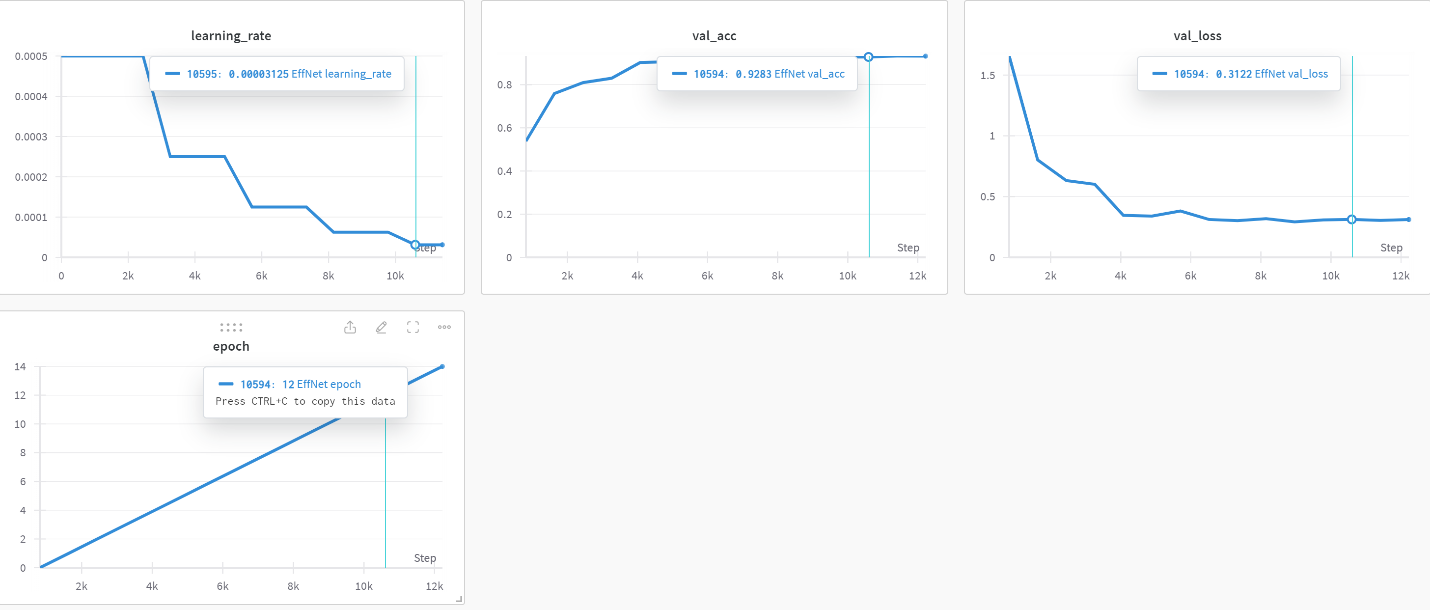
\includegraphics[width=16cm]{images/10.png}
\caption{Метрики процесса обучения модели, автоматически созданные с помощью библиотеки \foreignlanguage{english}{wandb}}
\label{fig:10}
\end{figure}

\subsection{Возможные улучшения}
\hspace{1cm}Для улучшения результатов предлагается увеличить размер датасета, использовать более сложные архитектурыии применять
методы регуляризации, такие как dropout. На датасете уже из 246 марок автомобиля модель показала точность результата
84,5\%. Но при этом при наборе данных на реальных фотографиях проявила более точные результаты.

\begin{figure}[H]
\centering
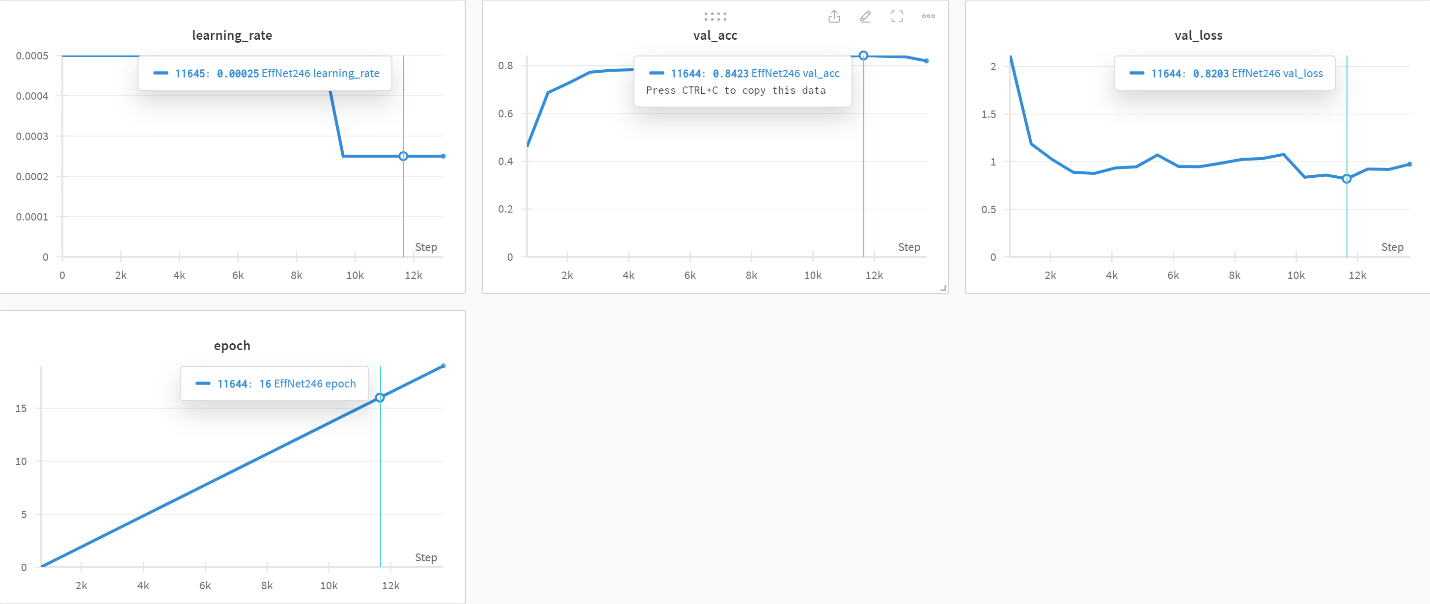
\includegraphics[width=16cm]{images/11.png}
\caption{Метрики процесса обучения модели, автоматически созданные с помощью библиотеки \foreignlanguage{english}{wandb}}
\label{fig:10}
\end{figure}

Теперь представимвсе модели на одном графике и обсудим их содержимое.

\begin{figure}[H]
\centering
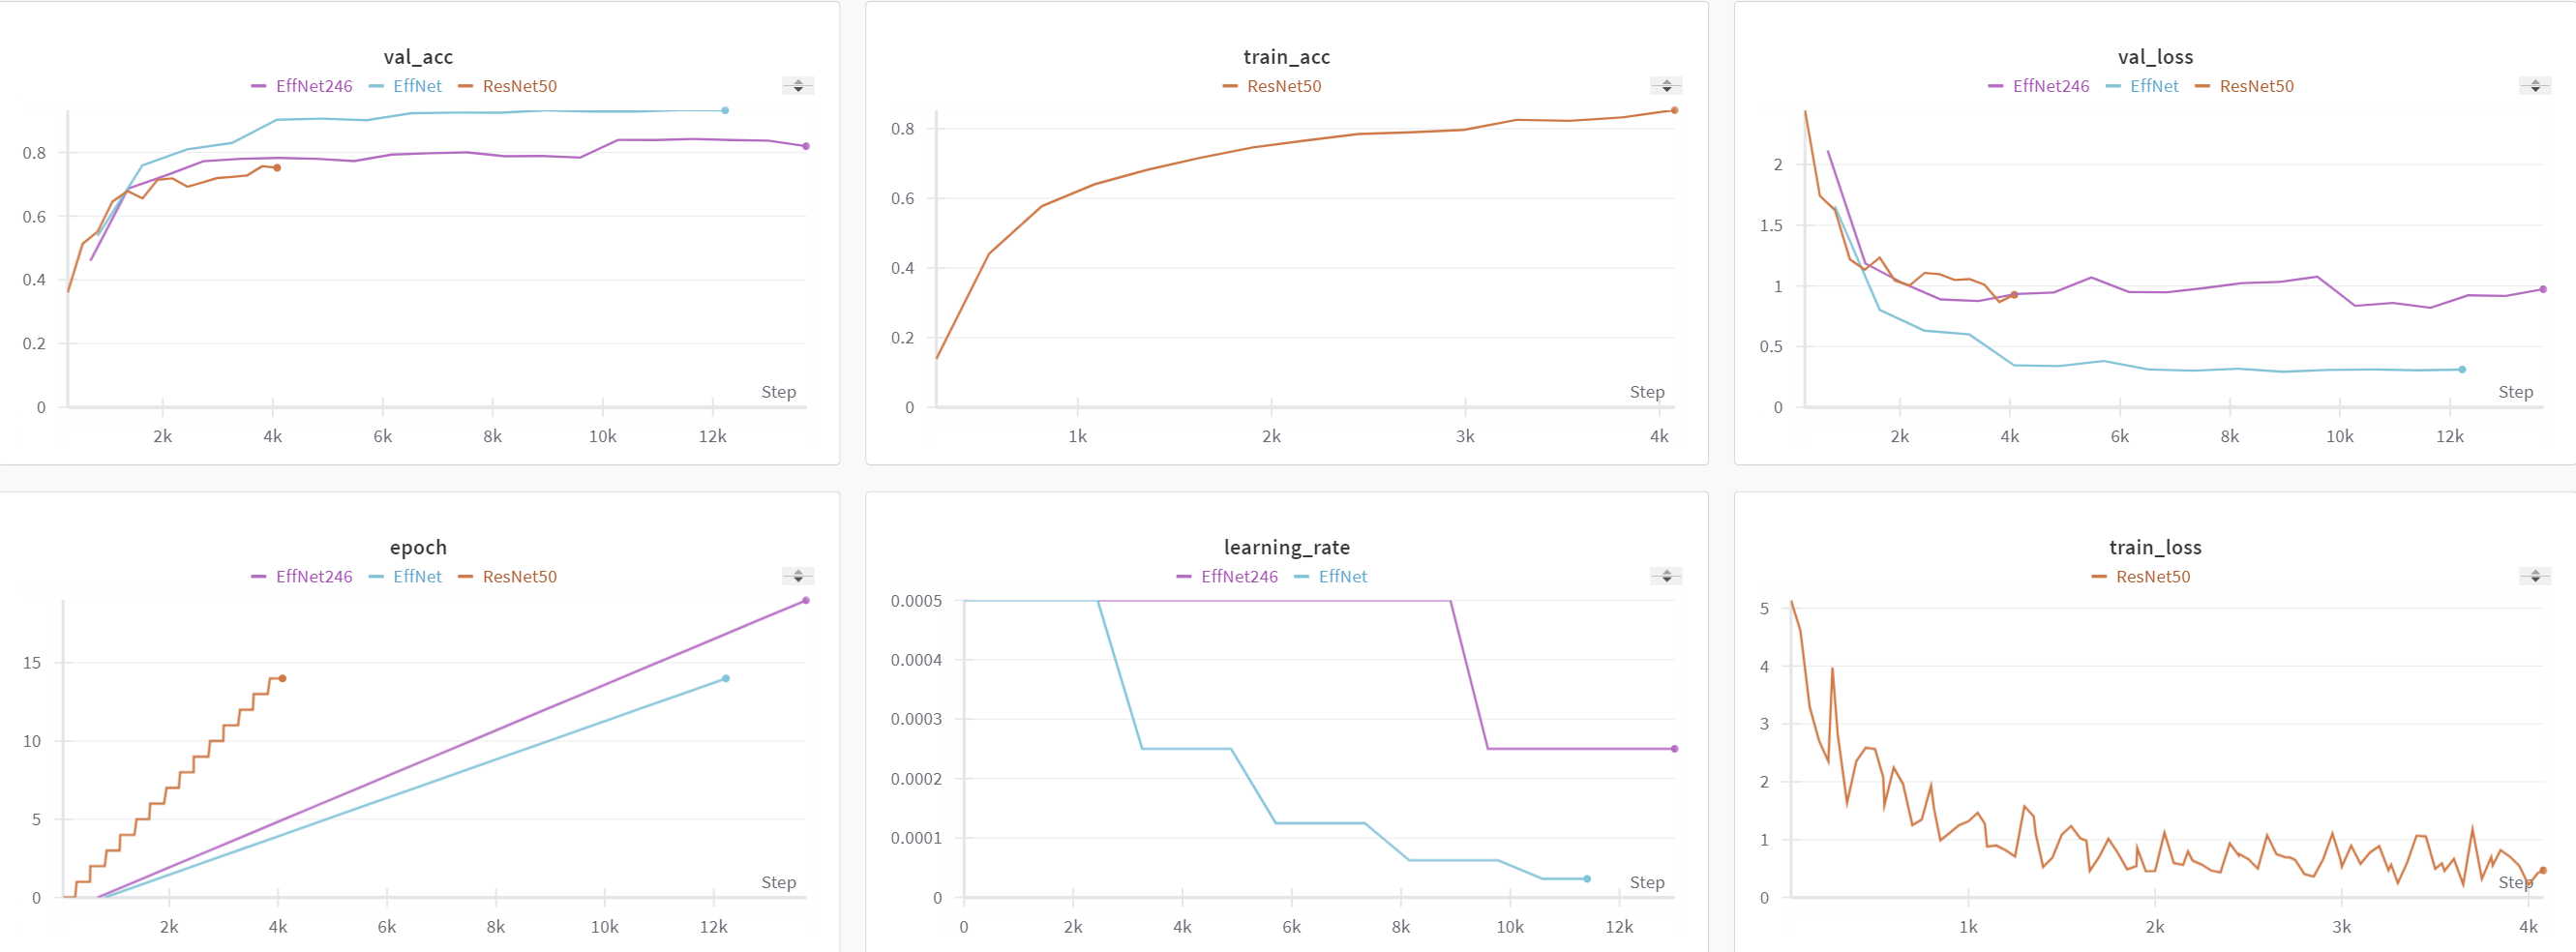
\includegraphics[width=\textwidth]{images/30.png}
\caption{Метрики процесса обучения всех моделей, автоматически созданные с помощью библиотеки \foreignlanguage{english}{wandb}}
\label{fig:10}
\end{figure}

\textbf{Описание графиков:}

\begin{itemize}
    \item \textbf{График \textit{val\_acc} (верхний левый)}: Отображает точность (accuracy) на валидационном наборе данных для моделей EffNet246, EffNet и ResNet50 по мере увеличения числа шагов (steps) или эпох (epochs). Видно, что точность на валидационном наборе увеличивается по мере обучения модели, достигая высоких значений.
    \item \textbf{График \textit{train\_acc} (верхний центральный)}: Отображает точность на тренировочном наборе данных для модели ResNet50 по мере увеличения числа шагов. Точность на тренировочном наборе также увеличивается по мере обучения, достигая значений около 0.85.
    \item \textbf{График \textit{val\_loss} (верхний правый)}: Отображает значение функции потерь (loss) на валидационном наборе данных для моделей EffNet246, EffNet и ResNet50 по мере увеличения числа шагов. Значение потерь уменьшается по мере обучения модели, что указывает на улучшение её производительности на валидационных данных.
    \item \textbf{График \textit{epoch} (нижний левый)}: Отображает номер текущей эпохи для моделей EffNet246, EffNet и ResNet50 по мере увеличения числа шагов. Видно, что обучение моделей продолжается до 15-й эпохи.
    \item \textbf{График \textit{learning\_rate} (нижний центральный)}: Отображает изменение скорости обучения (learning rate) для моделей EffNet246 и EffNet по мере увеличения числа шагов. Видно, что скорость обучения уменьшается ступенчато в течение обучения.
    \item \textbf{График \textit{train\_loss} (нижний правый)}: Отображает значение функции потерь на тренировочном наборе данных для модели ResNet50 по мере увеличения числа шагов. Значение потерь на тренировочных данных снижается, что указывает на то, что модель обучается правильно. Рассчитывайте по этой формуле:
\[
J(W, b) = -\frac{1}{m} \sum_{i=1}^{m} \left( y_i \log(\hat{y}_i) + (1-y_i) \log(1-\hat{y}_i) \right)
\]
где \( m \) - количество примеров в обучающей выборке, \( y_i \) - истинная метка класса для \( i \)-го примера, \( \hat{y}_i \) - предсказанная моделью вероятность принадлежности к классу.

\end{itemize}

Эти графики вместе позволяют анализировать процесс обучения моделей:
\begin{itemize}
    \item \textbf{Сходимость}: Уменьшение функции потерь на тренировочных и валидационных данных указывает на то, что модели успешно обучаются.
    \item \textbf{Обучение и валидация}: Сравнение точности и потерь на тренировочных и валидационных данных позволяет оценить, не происходит ли переобучение моделей. Если валидационные метрики (точность и потери) сильно отличаются от тренировочных, это может указывать на переобучение.
    \item \textbf{Эффективность моделей}: Высокие значения точности и низкие значения потерь показывают, что модели достигают хорошей производительности.
\end{itemize}

\section[Использование модели]{\textbf{Использование модели}}
\ \ В данной главе рассмотрим использование модели и выявим несколько закономерностей. Протестируем фотографии разных
размеров на двух моделях:
\begin{itemize}
    \item  \foreignlanguage{english}{EfficientNet} на датасете из 196 марок 
    \item  \foreignlanguage{english}{EfficientNet} на датасете из 246 марок 
\end{itemize}

Начнем с простого. В датасете есть Ferrari 458 Italia Coupe 2012, протестируем модель на фотографии Ferrari 458 Italia Coupe 2013 

\begin{figure}[H]
\centering
\begin{minipage}{0.49\textwidth}
  \centering
  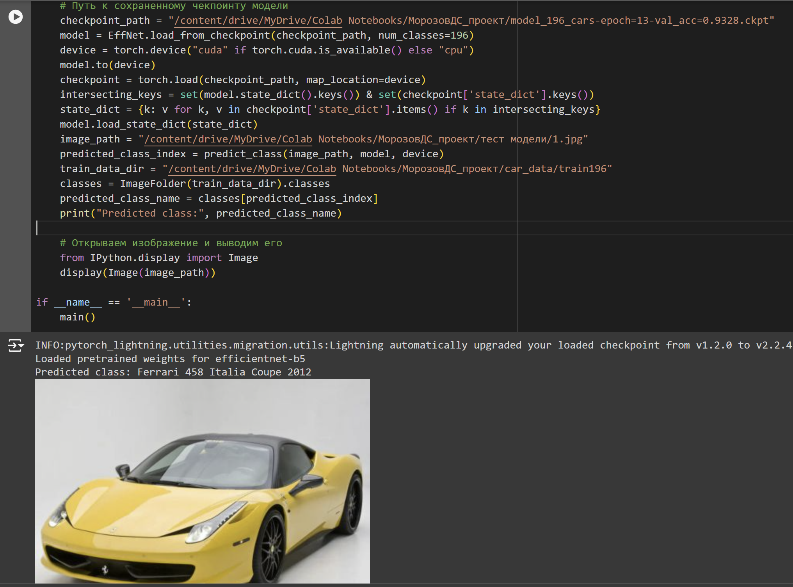
\includegraphics[height=5.6cm]{images/12.png}  
  \caption{Демонстрация работы модели \foreignlanguage{english}{EfficientNet} на датасете из 196 марок}
  \label{fig:12}
\end{minipage}
\hfill
\begin{minipage}{0.49\textwidth}
  \centering
  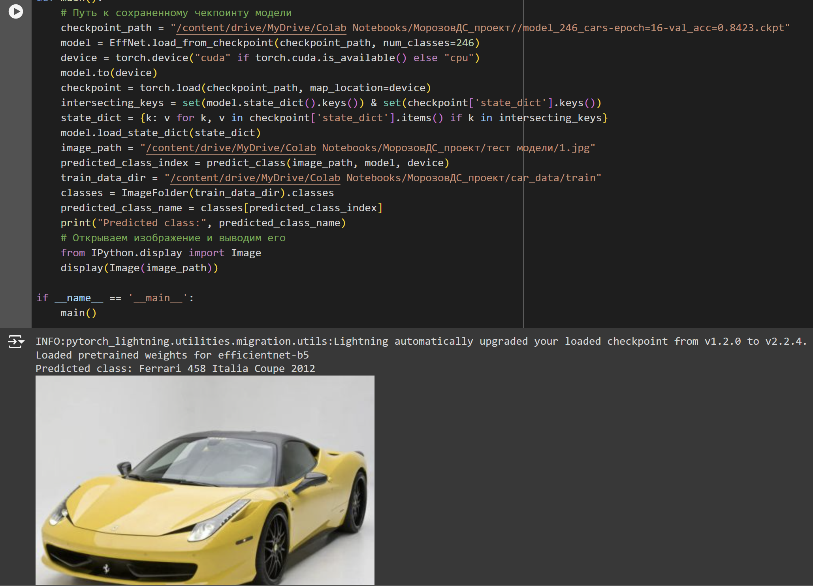
\includegraphics[height=5.6cm]{images/13.png}  
  \caption{Демонстрация работы модели \foreignlanguage{english}{EfficientNet} на датасете из 246 марок}
  \label{fig:13}
\end{minipage}
\end{figure}

\noindent Обе модели легко справились с этой задачей. 

Усложним задачу. Возьмем фотографию из auto.ru. А так же возьмем по новее год 2015 (так как в датасете марки автомобилей максимум 2012 год).
\begin{figure}[H]
\centering
\begin{minipage}{0.49\textwidth}
  \centering
  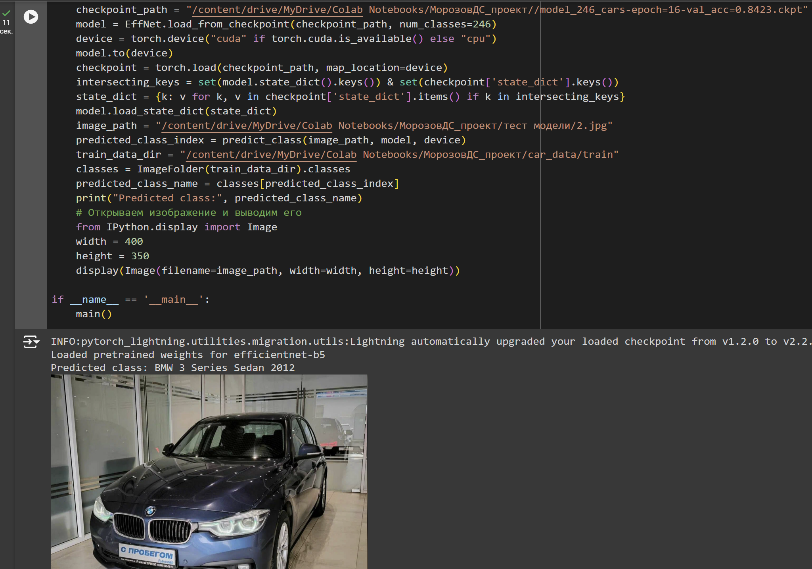
\includegraphics[height=5.6cm]{images/14.png}  
  \caption{Демонстрация работы модели \foreignlanguage{english}{EfficientNet} на датасете из 196 марок}
  \label{fig:12}
\end{minipage}
\hfill
\begin{minipage}{0.49\textwidth}
  \centering
  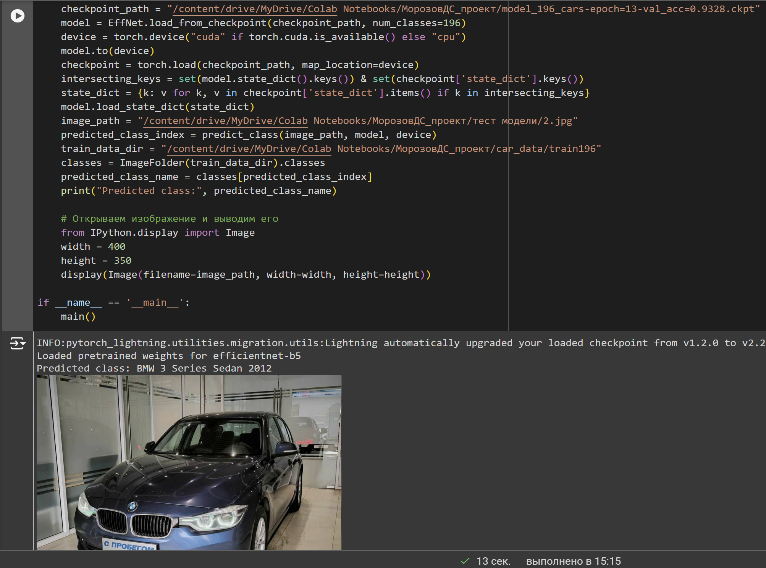
\includegraphics[height=5.6cm]{images/15.png}  
  \caption{Демонстрация работы модели \foreignlanguage{english}{EfficientNet} на датасете из 246 марок}
  \label{fig:13}
\end{minipage}
\end{figure}

\noindent Все две модели справились.

\noindent Усложним задачу. Возьмем фотографию из auto.ru. И возьмем год 2022

\begin{figure}[H]
\centering
\begin{minipage}{0.49\textwidth}
  \centering
  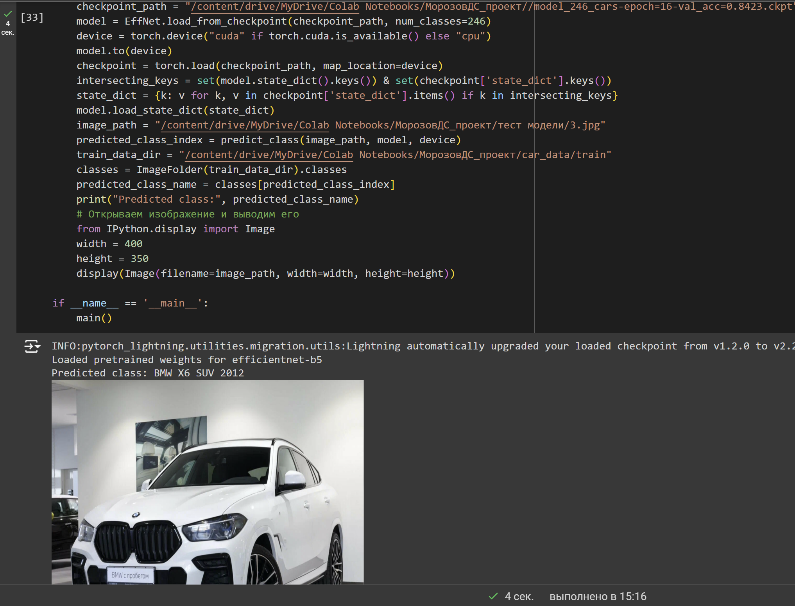
\includegraphics[height=7.1cm]{images/16.png}  
  \caption{Демонстрация работы модели \foreignlanguage{english}{EfficientNet} на датасете из 196 марок}
  \label{fig:12}
\end{minipage}
\hfill
\begin{minipage}{0.49\textwidth}
  \centering
  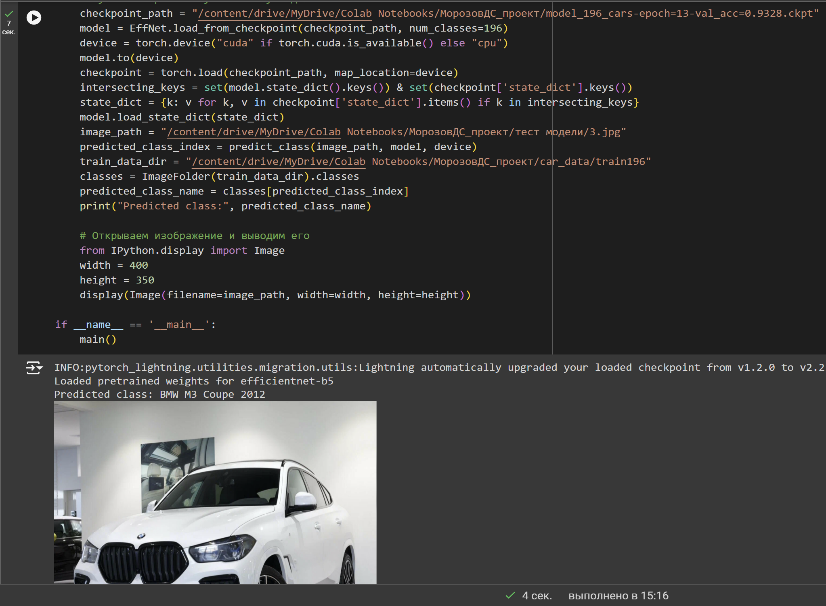
\includegraphics[height=7.1cm]{images/17.png}  
  \caption{Демонстрация работы модели \foreignlanguage{english}{EfficientNet} на датасете из 246 марок}
  \label{fig:13}
\end{minipage}
\end{figure}

Здесь уже видим, что модель, у которой точность хоть и выше выдала не верный предикт, но тем времени модель с большим количеством марок и меньшей точностью справилась правильно.

\noindentТеперь можно попробовать сфоткать автомобиль на улице и загрузить

\begin{figure}[H]
\centering
\begin{minipage}{0.49\textwidth}
  \centering
  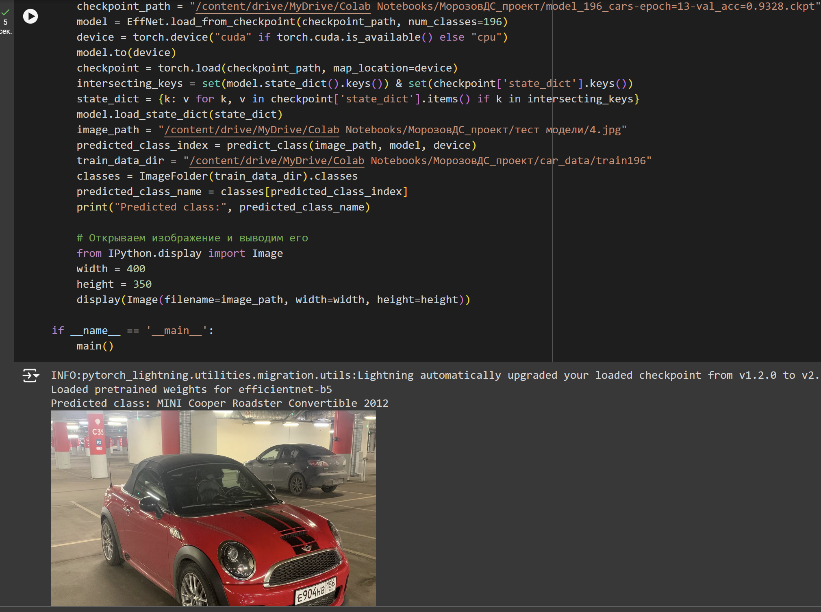
\includegraphics[height=7.1cm]{images/18.png}  
  \caption{Демонстрация работы модели \foreignlanguage{english}{EfficientNet} на датасете из 196 марок}
  \label{fig:12}
\end{minipage}
\hfill
\begin{minipage}{0.49\textwidth}
  \centering
  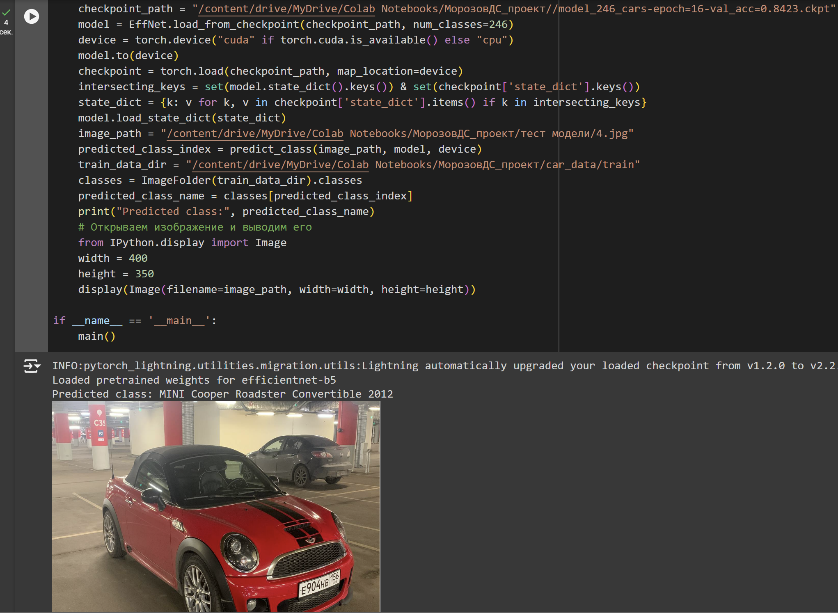
\includegraphics[height=7.1cm]{images/19.png}  
  \caption{Демонстрация работы модели \foreignlanguage{english}{EfficientNet} на датасете из 246 марок}
  \label{fig:13}
\end{minipage}
\end{figure}

\noindentВсе две модели справились отлично.

\noindentПопробуем сфоткать для модели более сложный кадр.

\begin{figure}[H]
\centering
\begin{minipage}{0.49\textwidth}
  \centering
  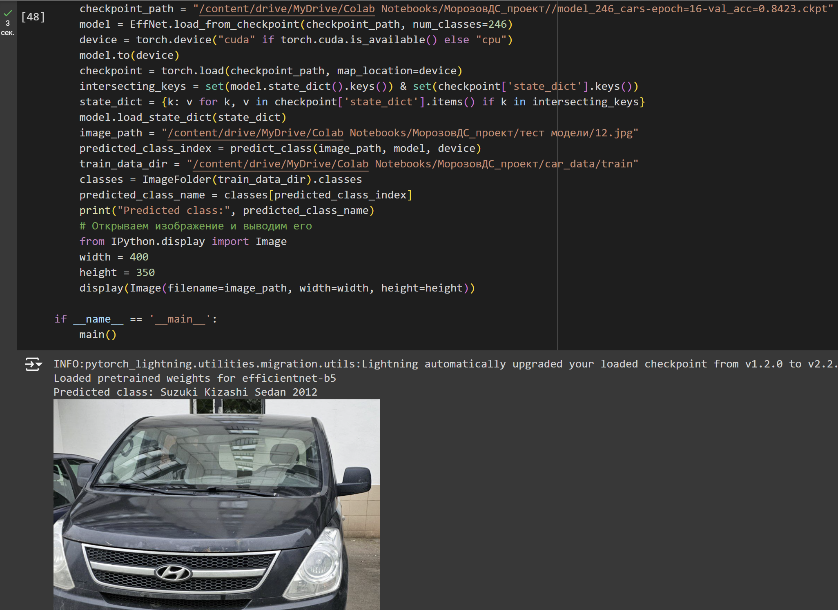
\includegraphics[height=7.1cm]{images/20.png}  
  \caption{Демонстрация работы модели \foreignlanguage{english}{EfficientNet} на датасете из 196 марок}
  \label{fig:12}
\end{minipage}
\hfill
\begin{minipage}{0.49\textwidth}
  \centering
  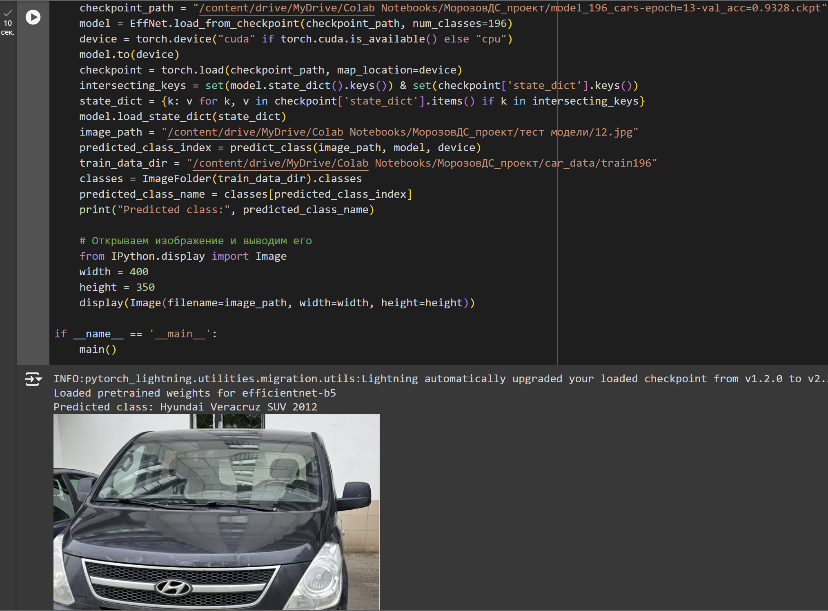
\includegraphics[height=7.1cm]{images/21.png}  
  \caption{Демонстрация работы модели \foreignlanguage{english}{EfficientNet} на датасете из 246 марок}
  \label{fig:13}
\end{minipage}
\end{figure}

Мы можем заметить, что модель с 93\% точностью правильно предиктовала название автомобиля в то время, как модель с более большим датасетом сделала это не корректно.\\
\noindentВот еще несколько тестов:

\begin{figure}[H]
\centering
\begin{minipage}{0.49\textwidth}
  \centering
  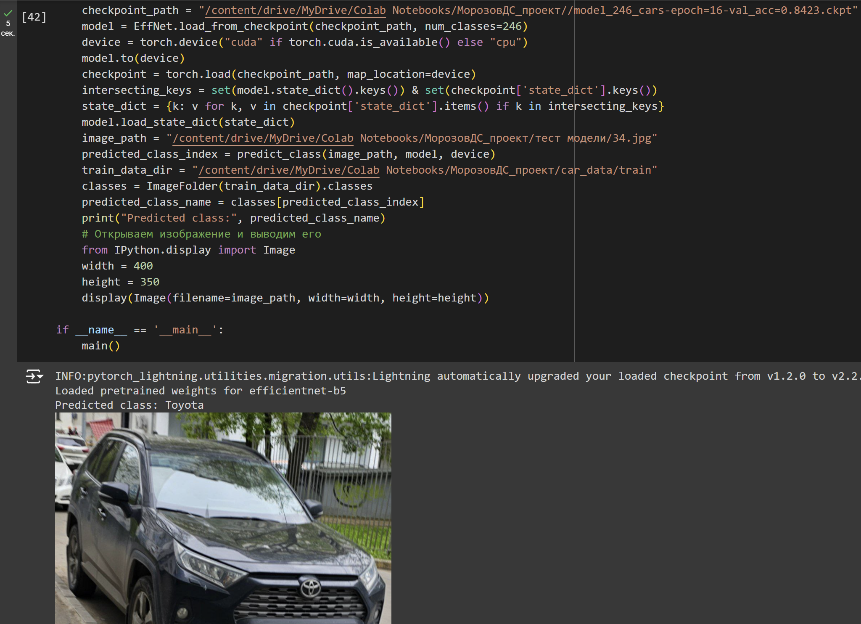
\includegraphics[height=6cm]{images/22.png}  
  \caption{Демонстрация работы модели \foreignlanguage{english}{EfficientNet} на датасете из 196 марок}
  \label{fig:12}
\end{minipage}
\hfill
\begin{minipage}{0.49\textwidth}
  \centering
  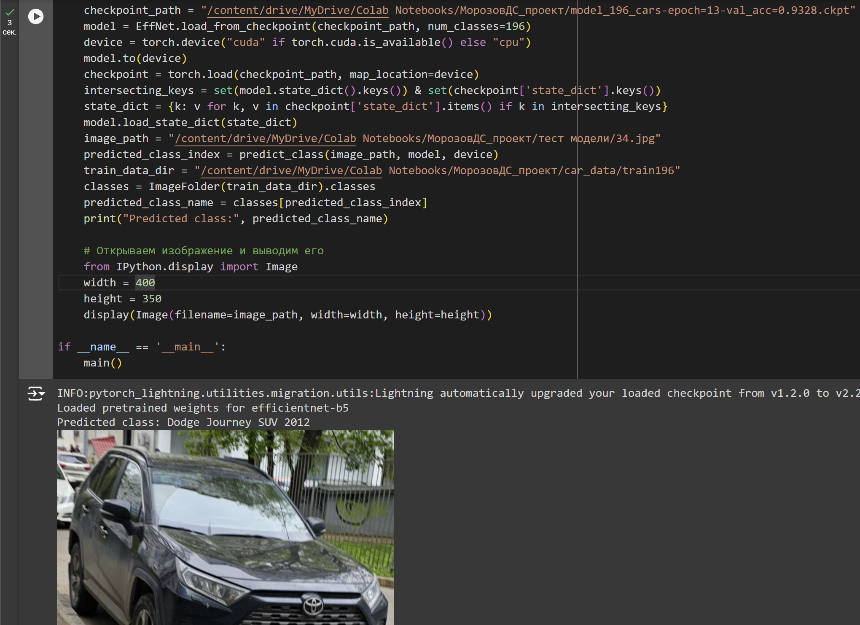
\includegraphics[height=6cm]{images/23.png}  
  \caption{Демонстрация работы модели \foreignlanguage{english}{EfficientNet} на датасете из 246 марок}
  \label{fig:13}
\end{minipage}
\end{figure}\begin{figure}[H]
\centering
\begin{minipage}{0.49\textwidth}
  \centering
  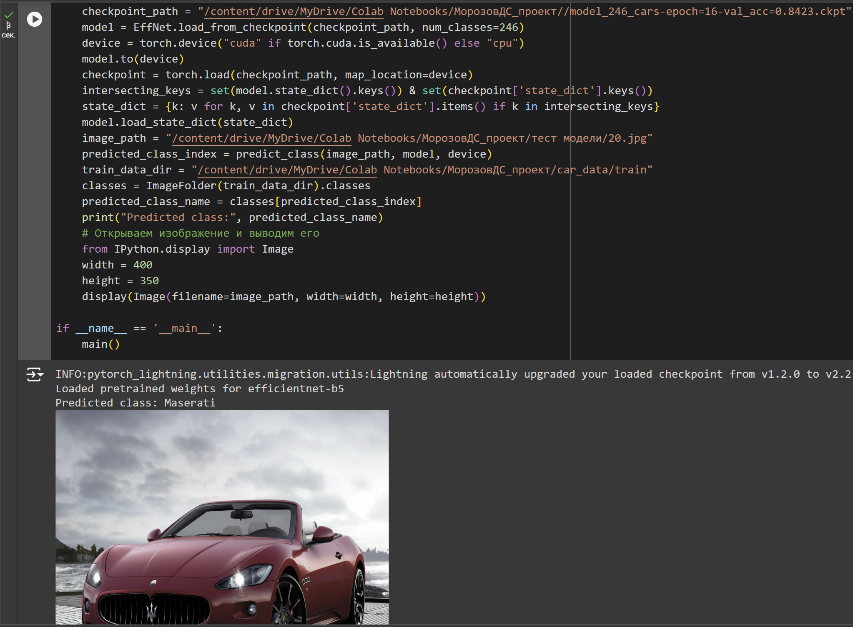
\includegraphics[height=6cm]{images/24.png}  
  \caption{Демонстрация работы модели \foreignlanguage{english}{EfficientNet} на датасете из 196 марок}
  \label{fig:12}
\end{minipage}
\hfill
\begin{minipage}{0.49\textwidth}
  \centering
  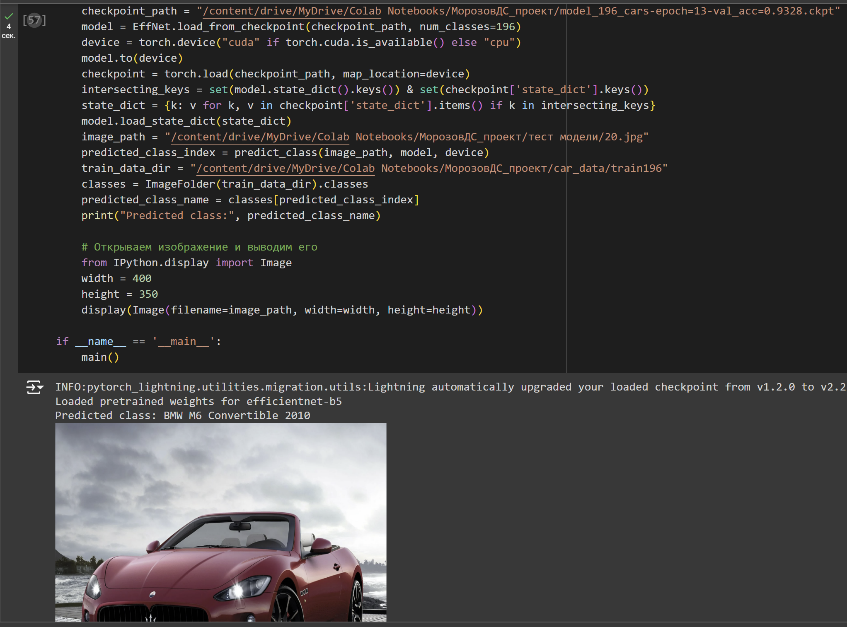
\includegraphics[height=6cm]{images/25.png}  
  \caption{Демонстрация работы модели \foreignlanguage{english}{EfficientNet} на датасете из 246 марок}
  \label{fig:13}
\end{minipage}
\end{figure}\begin{figure}[H]
\centering
\begin{minipage}{0.49\textwidth}
  \centering
  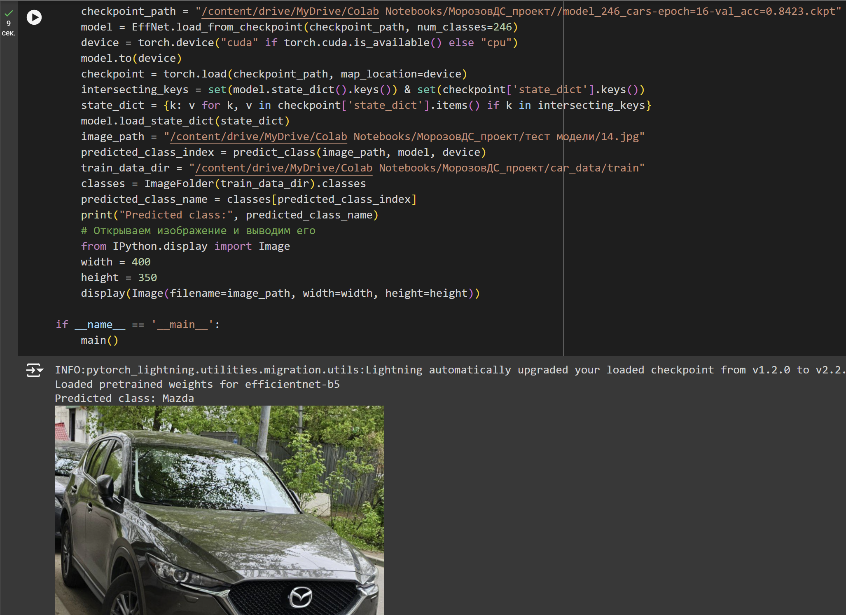
\includegraphics[height=7.1cm]{images/26.png}  
  \caption{Демонстрация работы модели \foreignlanguage{english}{EfficientNet} на датасете из 196 марок}
  \label{fig:12}
\end{minipage}
\hfill
\begin{minipage}{0.49\textwidth}
  \centering
  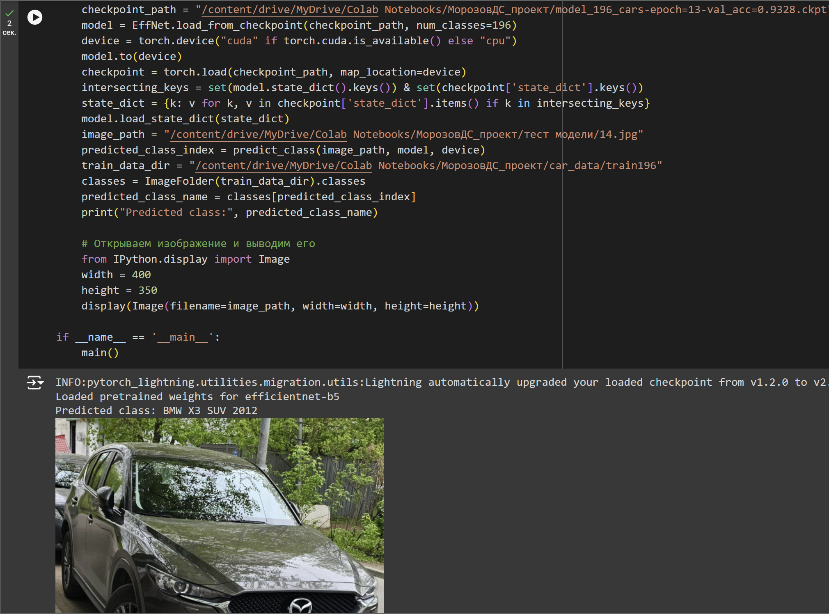
\includegraphics[height=7.1cm]{images/27.png}  
  \caption{Демонстрация работы модели \foreignlanguage{english}{EfficientNet} на датасете из 246 марок}
  \label{fig:13}
\end{minipage}
\end{figure}\begin{figure}[H]
\centering
\begin{minipage}{0.49\textwidth}
  \centering
  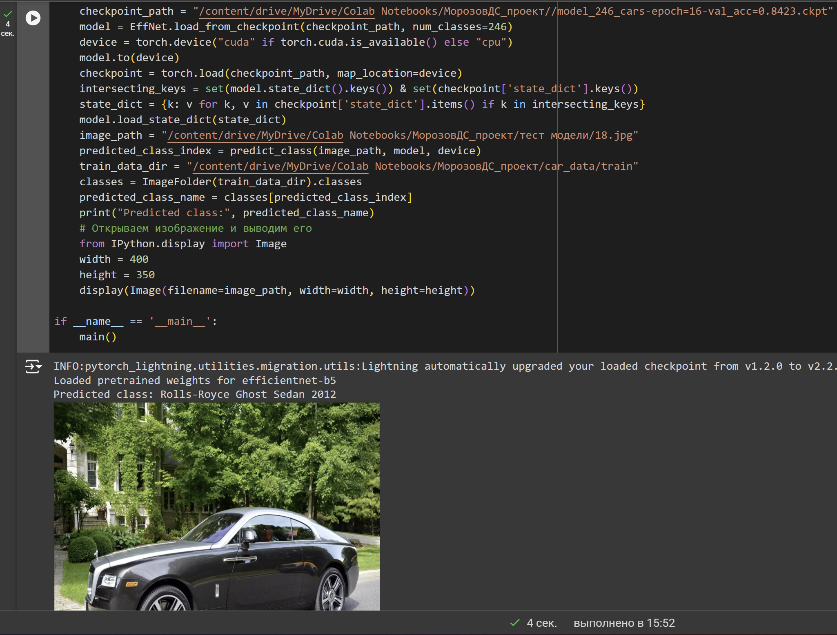
\includegraphics[height=7.2cm]{images/28.png}  
  \caption{Демонстрация работы модели \foreignlanguage{english}{EfficientNet} на датасете из 196 марок}
  \label{fig:12}
\end{minipage}
\hfill
\begin{minipage}{0.49\textwidth}
  \centering
  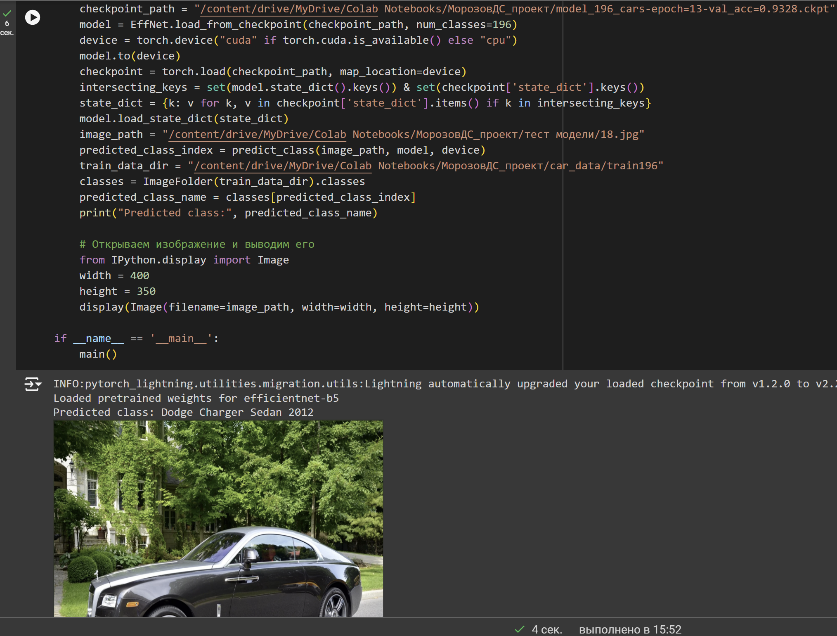
\includegraphics[height=7.2cm]{images/29.png}  
  \caption{Демонстрация работы модели \foreignlanguage{english}{EfficientNet} на датасете из 246 марок}
  \label{fig:13}
\end{minipage}
\end{figure}

Из этих тестов мы можем сделать вывод, что датасет влияет на предиктовку больше, чем точность модели.


\section[Заключение]{\textbf{Заключение}}
Проект показал, что глубокие нейронные сети могут эффективно решать задачу распознавания марок автомобилей по
фотографиям. Достигнутые результаты подтверждают правильность выбранного подхода, однако есть возможности для
дальнейшего улучшения модели.

В ходе проекта была разработана и обучена модель нейронной сети для классификации изображений автомобилей. Дальнейшие
исследования и улучшения могут включать более сложные методы аугментации данных, более новую архитектуру модели такие
как EfficientNet\foreignlanguage{english}{B}7 настройку гиперпараметров и расширение датасета для улучшения
производительности модели.
\newpage
\nocite{*} % Включить все записи из библиографии
\printbibliography[title={Список использованных источников}] % Заголовок списка литературы

\end{document}